\begin{frame}{Data Explanation}
\begin{itemize}
 \item 1514 MD Anderson patients who had brainmets from breast cancer
 \item 90 covariates
 \begin{itemize}
  \item Missingness from 0 to 65\%
 \end{itemize}

\end{itemize}
\begin{table}[ !ht]
\centering
\begin{tabular}{|c|c|}
\hline
Type                                                                            & Example                                                                       \\ \hline
Subject data                                                                    & Age range, race, date of birth                                                \\ \hline
Cancer data                                                                     & TNM staging, type, receptor status                                            \\ \hline
\begin{tabular}[c]{@{}c@{}}Pre brain mets\\ data\end{tabular}                   & Treatment types                                                               \\ \hline
\begin{tabular}[c]{@{}c@{}}Post brain mets\\ clinical observations\end{tabular} & Seizures, headache, nasuea                                                    \\ \hline
\begin{tabular}[c]{@{}c@{}}Post brain mets\\ data\end{tabular}                  & \begin{tabular}[c]{@{}c@{}}Treatment type, \\ type of brain mets\end{tabular} \\ \hline
Survival data                                                                   & Survival time after brain mets, censoring indicator                           \\ \hline
\end{tabular}
\caption{Data Categories and Examples}
\label{table:cats}
\end{table}

\end{frame}

\begin{frame}{Important Covariates}
 \begin{table}[ !ht]
\centering
\adjustbox{max height=\dimexpr\textheight-5.5cm\relax,
           max width=\textwidth}{
\begin{tabular}{|c|c|c|}
\hline
Name        & \begin{tabular}[c]{@{}c@{}}Percent \\ Missing\end{tabular} & Meaning                                                                                                                                             \\ \hline
hrher2      & 5                                                        & \begin{tabular}[c]{@{}c@{}}Categorical variable: The hormonal receptor and \\ HER2 receptor status of the subject\end{tabular}                      \\ \hline
agebrainmet & 0                                                          & Indicator: Age greater or less than 60 at time of brain mets                                                                                        \\ \hline
timedx      & 1                                                         & \begin{tabular}[c]{@{}c@{}}Indicator: Time (years) from breast cancer diagnosis to brain\\ mets diagnosis greater or less than 6 years\end{tabular} \\ \hline
site5       & 1                                                        & Indicator: First metastasis was to brain                                                                                                            \\ \hline
race2       & 0                                                          & Categorical: White, Black, Hispanic, other                                                                                                          \\ \hline
priorn      & 0                                                          & \begin{tabular}[c]{@{}c@{}}Indicator: Number of prior treatments in metastatic setting \\ before brain mets\end{tabular}                            \\ \hline
braintype   & 4                                                        & Categorical: Single, multiple, Leptomeningeal disease                                                                                               \\ \hline
controlled  & 12                                                        & Indicator: Extracranial progression of brain mets                                                                                                   \\ \hline
capeothno   & 18                                                        & \begin{tabular}[c]{@{}c@{}}Indicator: Capecitabine, other, or no chemotheraputic\\ treatment. Treatment variable 1\end{tabular}                     \\ \hline
lapatrasno  & 18                                                        & \begin{tabular}[c]{@{}c@{}}Indicator: Lapatinib, Trastuzumab, or no HER2 treatment.\\ Treatment variable 2\end{tabular}                             \\ \hline
os          & 0                                                          & Overall survival (months)                                                                                                                           \\ \hline
dead        & 0                                                          & Indicator: death indicator                                                                                                                          \\ \hline
her2        & 10                                                        & Indicator: HER2 receptor status                                                                                                                     \\ \hline
\end{tabular}
}
\caption{Table of important covariates to be used in the analysis}
\label{table:importantvars}

\end{table}
\end{frame}

\begin{frame}{Visualization of Missingness}
 \begin{figure}[h!]
  \centering
    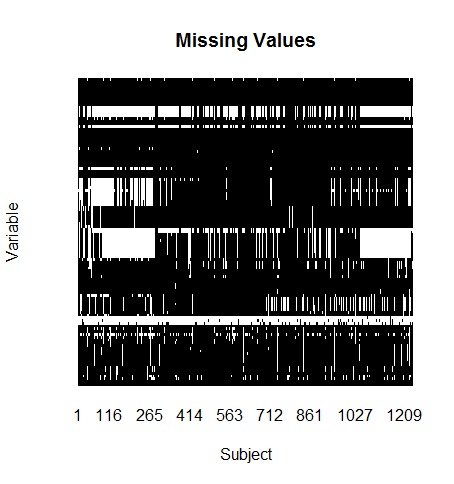
\includegraphics[width=0.8\textwidth]{missingvalues_plot.png}
  \caption{Visualization of missingness in the cancer dataset}
\label{fig:missingplot}
\medskip
\small
Along the horizontal axis is the subject, and the vertical axis is the covariates. \textcolor{green}{Green} denotes observed values whereas \textcolor{red}{red} is missing. The covariates with the highest missingness are three genetic measures, as well as some clinical assessments.
\end{figure}
\end{frame}

